% Graphic for TeX using PGF
% Title: /Users/bubel/Documents/Teaching/Lectures/PP/prgprd/Lectures/objmodel.dia
% Creator: Dia v0.97.1
% CreationDate: Fri Nov 19 11:05:10 2010
% For: bubel
% \usepackage{tikz}
% The following commands are not supported in PSTricks at present
% We define them conditionally, so when they are implemented,
% this pgf file will use them.
\ifx\du\undefined
  \newlength{\du}
\fi
\setlength{\du}{15\unitlength}
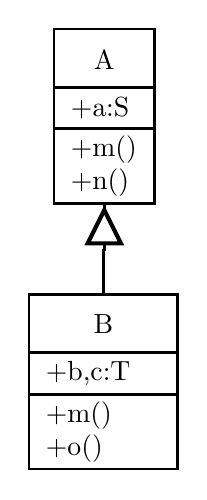
\begin{tikzpicture}
\pgftransformxscale{1.000000}
\pgftransformyscale{-1.000000}
\definecolor{dialinecolor}{rgb}{0.000000, 0.000000, 0.000000}
\pgfsetstrokecolor{dialinecolor}
\definecolor{dialinecolor}{rgb}{1.000000, 1.000000, 1.000000}
\pgfsetfillcolor{dialinecolor}
\pgfsetlinewidth{1pt}
\pgfsetdash{}{0pt}
\definecolor{dialinecolor}{rgb}{1.000000, 1.000000, 1.000000}
\pgfsetfillcolor{dialinecolor}
\fill (14.300000\du,5.900000\du)--(14.300000\du,7.300000\du)--(16.725000\du,7.300000\du)--(16.725000\du,5.900000\du)--cycle;
\definecolor{dialinecolor}{rgb}{0.000000, 0.000000, 0.000000}
\pgfsetstrokecolor{dialinecolor}
\draw (14.300000\du,5.900000\du)--(14.300000\du,7.300000\du)--(16.725000\du,7.300000\du)--(16.725000\du,5.900000\du)--cycle;
% setfont left to latex
\definecolor{dialinecolor}{rgb}{0.000000, 0.000000, 0.000000}
\pgfsetstrokecolor{dialinecolor}
\node at (15.512500\du,6.650000\du){A};
\definecolor{dialinecolor}{rgb}{1.000000, 1.000000, 1.000000}
\pgfsetfillcolor{dialinecolor}
\fill (14.300000\du,7.300000\du)--(14.300000\du,8.300000\du)--(16.725000\du,8.300000\du)--(16.725000\du,7.300000\du)--cycle;
\definecolor{dialinecolor}{rgb}{0.000000, 0.000000, 0.000000}
\pgfsetstrokecolor{dialinecolor}
\draw (14.300000\du,7.300000\du)--(14.300000\du,8.300000\du)--(16.725000\du,8.300000\du)--(16.725000\du,7.300000\du)--cycle;
% setfont left to latex
\definecolor{dialinecolor}{rgb}{0.000000, 0.000000, 0.000000}
\pgfsetstrokecolor{dialinecolor}
\node[anchor=west] at (14.450000\du,7.8000000\du){+a:S};
\definecolor{dialinecolor}{rgb}{1.000000, 1.000000, 1.000000}
\pgfsetfillcolor{dialinecolor}
\fill (14.300000\du,8.300000\du)--(14.300000\du,10.100000\du)--(16.725000\du,10.100000\du)--(16.725000\du,8.300000\du)--cycle;
\definecolor{dialinecolor}{rgb}{0.000000, 0.000000, 0.000000}
\pgfsetstrokecolor{dialinecolor}
\draw (14.300000\du,8.300000\du)--(14.300000\du,10.100000\du)--(16.725000\du,10.100000\du)--(16.725000\du,8.300000\du)--cycle;
% setfont left to latex
\definecolor{dialinecolor}{rgb}{0.000000, 0.000000, 0.000000}
\pgfsetstrokecolor{dialinecolor}
\node[anchor=west] at (14.450000\du,8.800000\du){+m()};
% setfont left to latex
\definecolor{dialinecolor}{rgb}{0.000000, 0.000000, 0.000000}
\pgfsetstrokecolor{dialinecolor}
\node[anchor=west] at (14.450000\du,9.600000\du){+n()};
\pgfsetlinewidth{1pt}
\pgfsetdash{}{0pt}
\definecolor{dialinecolor}{rgb}{1.000000, 1.000000, 1.000000}
\pgfsetfillcolor{dialinecolor}
\fill (13.700000\du,12.300000\du)--(13.700000\du,13.700000\du)--(17.280000\du,13.700000\du)--(17.280000\du,12.300000\du)--cycle;
\definecolor{dialinecolor}{rgb}{0.000000, 0.000000, 0.000000}
\pgfsetstrokecolor{dialinecolor}
\draw (13.700000\du,12.300000\du)--(13.700000\du,13.700000\du)--(17.280000\du,13.700000\du)--(17.280000\du,12.300000\du)--cycle;
% setfont left to latex
\definecolor{dialinecolor}{rgb}{0.000000, 0.000000, 0.000000}
\pgfsetstrokecolor{dialinecolor}
\node at (15.490000\du,13.0000\du){B};
\definecolor{dialinecolor}{rgb}{1.000000, 1.000000, 1.000000}
\pgfsetfillcolor{dialinecolor}
\fill (13.700000\du,13.700000\du)--(13.700000\du,14.700000\du)--(17.280000\du,14.700000\du)--(17.280000\du,13.700000\du)--cycle;
\definecolor{dialinecolor}{rgb}{0.000000, 0.000000, 0.000000}
\pgfsetstrokecolor{dialinecolor}
\draw (13.700000\du,13.700000\du)--(13.700000\du,14.700000\du)--(17.280000\du,14.700000\du)--(17.280000\du,13.700000\du)--cycle;
% setfont left to latex
\definecolor{dialinecolor}{rgb}{0.000000, 0.000000, 0.000000}
\pgfsetstrokecolor{dialinecolor}
\node[anchor=west] at (13.850000\du,14.200000\du){+b,c:T};
\definecolor{dialinecolor}{rgb}{1.000000, 1.000000, 1.000000}
\pgfsetfillcolor{dialinecolor}
\fill (13.700000\du,14.700000\du)--(13.700000\du,16.500000\du)--(17.280000\du,16.500000\du)--(17.280000\du,14.700000\du)--cycle;
\definecolor{dialinecolor}{rgb}{0.000000, 0.000000, 0.000000}
\pgfsetstrokecolor{dialinecolor}
\draw (13.700000\du,14.700000\du)--(13.700000\du,16.500000\du)--(17.280000\du,16.500000\du)--(17.280000\du,14.700000\du)--cycle;
% setfont left to latex
\definecolor{dialinecolor}{rgb}{0.000000, 0.000000, 0.000000}
\pgfsetstrokecolor{dialinecolor}
\node[anchor=west] at (13.850000\du,15.200000\du){+m()};
% setfont left to latex
\definecolor{dialinecolor}{rgb}{0.000000, 0.000000, 0.000000}
\pgfsetstrokecolor{dialinecolor}
\node[anchor=west] at (13.850000\du,16.000000\du){+o()};
\pgfsetlinewidth{1pt}
\pgfsetdash{}{0pt}
\pgfsetmiterjoin
\pgfsetbuttcap
{
\definecolor{dialinecolor}{rgb}{0.000000, 0.000000, 0.000000}
\pgfsetfillcolor{dialinecolor}
% was here!!!
\definecolor{dialinecolor}{rgb}{0.000000, 0.000000, 0.000000}
\pgfsetstrokecolor{dialinecolor}
\draw (15.512500\du,10.150262\du)--(15.512500\du,11.225131\du)--(15.490000\du,11.225131\du)--(15.490000\du,12.300000\du);
}
\definecolor{dialinecolor}{rgb}{0.000000, 0.000000, 0.000000}
\pgfsetstrokecolor{dialinecolor}
\draw (15.512500\du,11.062066\du)--(15.512500\du,11.225131\du)--(15.490000\du,11.225131\du)--(15.490000\du,12.300000\du);
\pgfsetmiterjoin
\definecolor{dialinecolor}{rgb}{1.000000, 1.000000, 1.000000}
\pgfsetfillcolor{dialinecolor}
\fill (15.912500\du,11.062066\du)--(15.512500\du,10.262066\du)--(15.112500\du,11.062066\du)--cycle;
\pgfsetlinewidth{0.100000\du}
\pgfsetdash{}{0pt}
\pgfsetmiterjoin
\definecolor{dialinecolor}{rgb}{0.000000, 0.000000, 0.000000}
\pgfsetstrokecolor{dialinecolor}
\draw (15.912500\du,11.062066\du)--(15.512500\du,10.262066\du)--(15.112500\du,11.062066\du)--cycle;
% setfont left to latex
\end{tikzpicture}
